\documentclass[margin=5mm, tikz]{standalone}
\usepackage[utf8x]{inputenc}
\usepackage{tikz}
\begin{document}
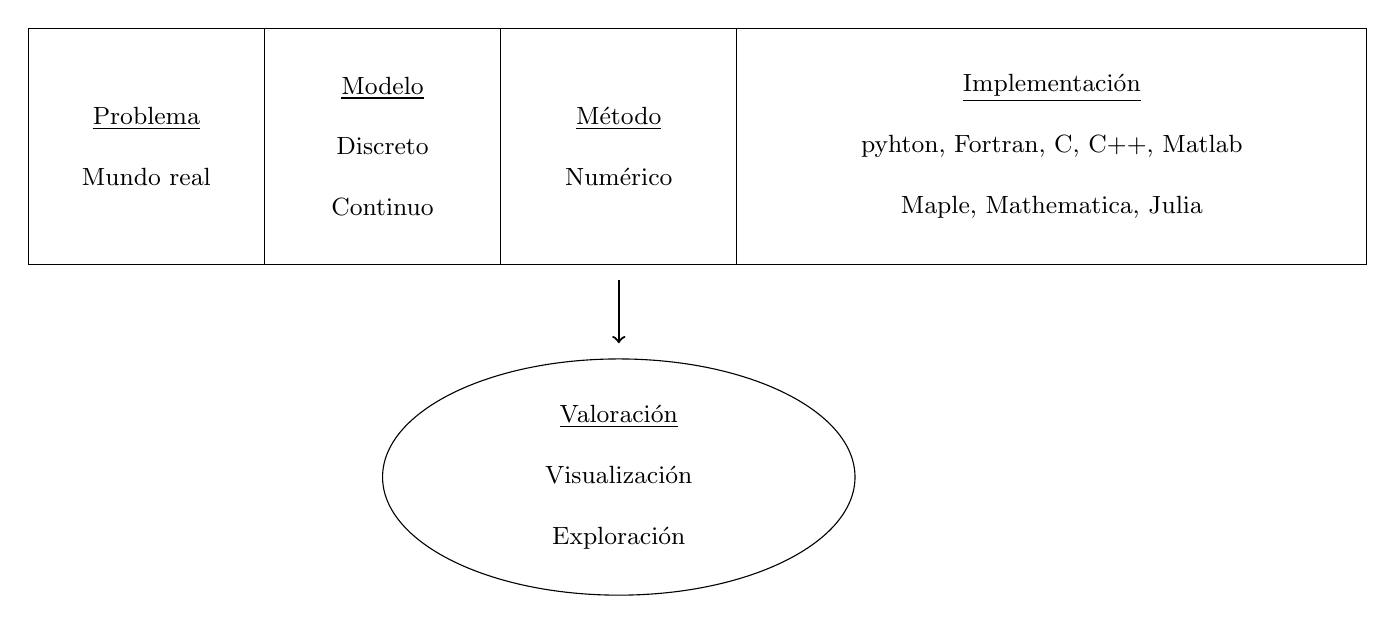
\begin{tikzpicture}[font = \small]

    \draw [align=center] (0, 0) rectangle (3, 3) node [pos=0.5] {\underline{Problema} \\ \\ Mundo real};

    \draw [align=center] (3, 0) rectangle (6, 3) node [pos=0.5] {\underline{Modelo} \\ \\ Discreto \\ \\ Continuo};

    \draw [align=center] (6, 0) rectangle (9, 3) node [pos=0.5] {\underline{Método} \\ \\ Numérico};

    \draw [align=center] (9, 0) rectangle (17, 3) node [pos=0.5] {\underline{Implementación} \\ \\ pyhton, Fortran, C, C++, Matlab \\ \\ Maple, Mathematica, Julia};

    \draw [align=center](7.5, -2.7) ellipse (3cm and 1.5cm) node {\underline{Valoración} \\ \\ Visualización \\ \\ Exploración};

    \draw[->, thick] (7.5, -0.2) -- (7.5, -1);
\end{tikzpicture}
\end{document}